\chapter{Конструкторский раздел}
\label{cha:design}

В данном разделе проектируется новая всячина.

\section{Архитектура всячины}

\subsection{Протестируем подпункт}
\subsubsection{А теперь подподпункт}


\paragraph{Проверка} параграфа. Вроде работает.
\paragraph{Вторая проверка} параграфа. Опять работает.

Вот.

\begin{itemize}
\item Это список с <<палочками>>.
\item Хотя он и по ГОСТ, но\dots
\end{itemize}

\begin{enumerate}
\item  Для списка, начинающегося с заглавной буквы, лучше список с цифрами.
\end{enumerate}

Формула \ref{F:F1} совершено бессмысленна.

%Кстати, при каких-то условиях <<удавалось>> получить двойный скобки вокруг номеров формул. Вопрос исследуется.

\begin{equation}
a= cb
\label{F:F1}
\end{equation}


Окружение \texttt{cases} опять работает (см. \ref{F:F2}), спасибо И. Короткову за исправления..


\begin{equation}
a= \begin{cases}
 3x + 5y + z, \mbox{если хорошо} \\
 7x - 2y + 4z, \mbox{если плохо}\\
 -6x + 3y + 2z, \mbox{если совсем плохо}
\end{cases}
\label{F:F2}
\end{equation}

\section{Подсистема всякой ерунды}

Культурная вставка dot-файлов через утилиту dot2tex (рис.~\ref{fig:fig02}).

\begin{figure}
  \centering
% [width=0.5\textwidth] --- регулировка ширины картинки
  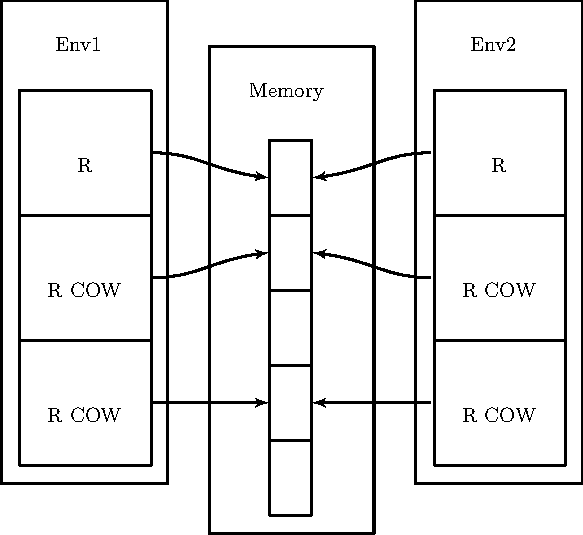
\includegraphics[width=.5\textwidth]{inc/dot/cow2}
  \caption{Рисунок}
  \label{fig:fig02}
\end{figure}


\subsection{Блок-схема всякой ерунды}

\subsubsection*{Кстати о заголовках}

У нас есть и \Code{subsubsection}. Только лучше её не нумеровать.

%%% Local Variables:
%%% mode: latex
%%% TeX-master: "rpz"
%%% End:
